\chapter{Solution Implementation}
\label{ch:implementation}

\section*{Introduction}
In this chapter, we provide a detailed step-by-step explanation of the implementation of the "CryptoEngine" demo. This demo showcases the use of cryptographic techniques to establish secure communication between two microcontrollers, specifically the STM32XX and STM32U545 MCUs.

\section{Demo Overview}
The following section outlines the sequence of operations involved in the "CryptoEngine" demo.
The steps are detailed in Table \ref{tab:authenticated_encryption_steps}:
\begin{longtable}{|c|p{6cm}|p{6cm}|}
\caption{Steps for "CryptoEngine" Demo} \label{tab:authenticated_encryption_steps} \\

\hline
\textbf{Step} & \textbf{Alice} & \textbf{Bob} \\
\hline
\endfirsthead

\multicolumn{3}{c}%
{{\bfseries \tablename\ \thetable{} -- continued from previous page}} \\
\hline
\textbf{Step} & \textbf{Alice} & \textbf{Bob} \\
\hline
\endhead

\hline \multicolumn{3}{|r|}{{Continued on next page}} \\ \hline
\endfoot

\hline
\endlastfoot

1 & Generate ECDSA Key Pair & Generate ECDSA Key Pair \\
  & \multicolumn{2}{p{12cm}|}{\textit{(ECDSA keys are used for creating and verifying digital signatures)}} \\
\hline
2 & Generate ECDH Key Pair & Generate ECDH Key Pair \\
  & \multicolumn{2}{p{12cm}|}{\textit{(ECDH keys are used for establishing a shared secret)}} \\
\hline
3 & Send ECDSA Public Key + Signature to Bob & Send ECDSA Public Key + Signature to Alice \\
\hline
4 & Verify Bob's Signature using his ECDSA Public Key & Verify Alice's Signature using her ECDSA Public Key \\
  & \multicolumn{2}{p{12cm}|}{\textit{(Ensures the authenticity of the participants)}} \\
\hline
5 & Send ECDH Public Key to Bob & Send ECDH Public Key to Alice \\
\hline
6 & Compute ECDH Shared Secret using own Private ECDH Key and Bob's Public ECDH Key & Compute ECDH Shared Secret using own Private ECDH Key and Alice's Public ECDH Key \\
  & \multicolumn{2}{p{12cm}|}{\textit{(Shared secret is used as the basis for deriving encryption keys)}} \\
\hline
7 & Derive AES GCM Key and IV from ECDH Shared Secret & Derive AES GCM Key and IV from ECDH Shared Secret \\
 
\hline
8 & Encrypt and Send Message using AES GCM & Decrypt and Verify Message using AES GCM \\
\hline
9 & Decrypt and Verify Response using AES GCM & Encrypt and Send Response using AES GCM \\
\hline

\end{longtable}

\section{Sequence Diagram}
\begin{figure}[H]
  \centering
  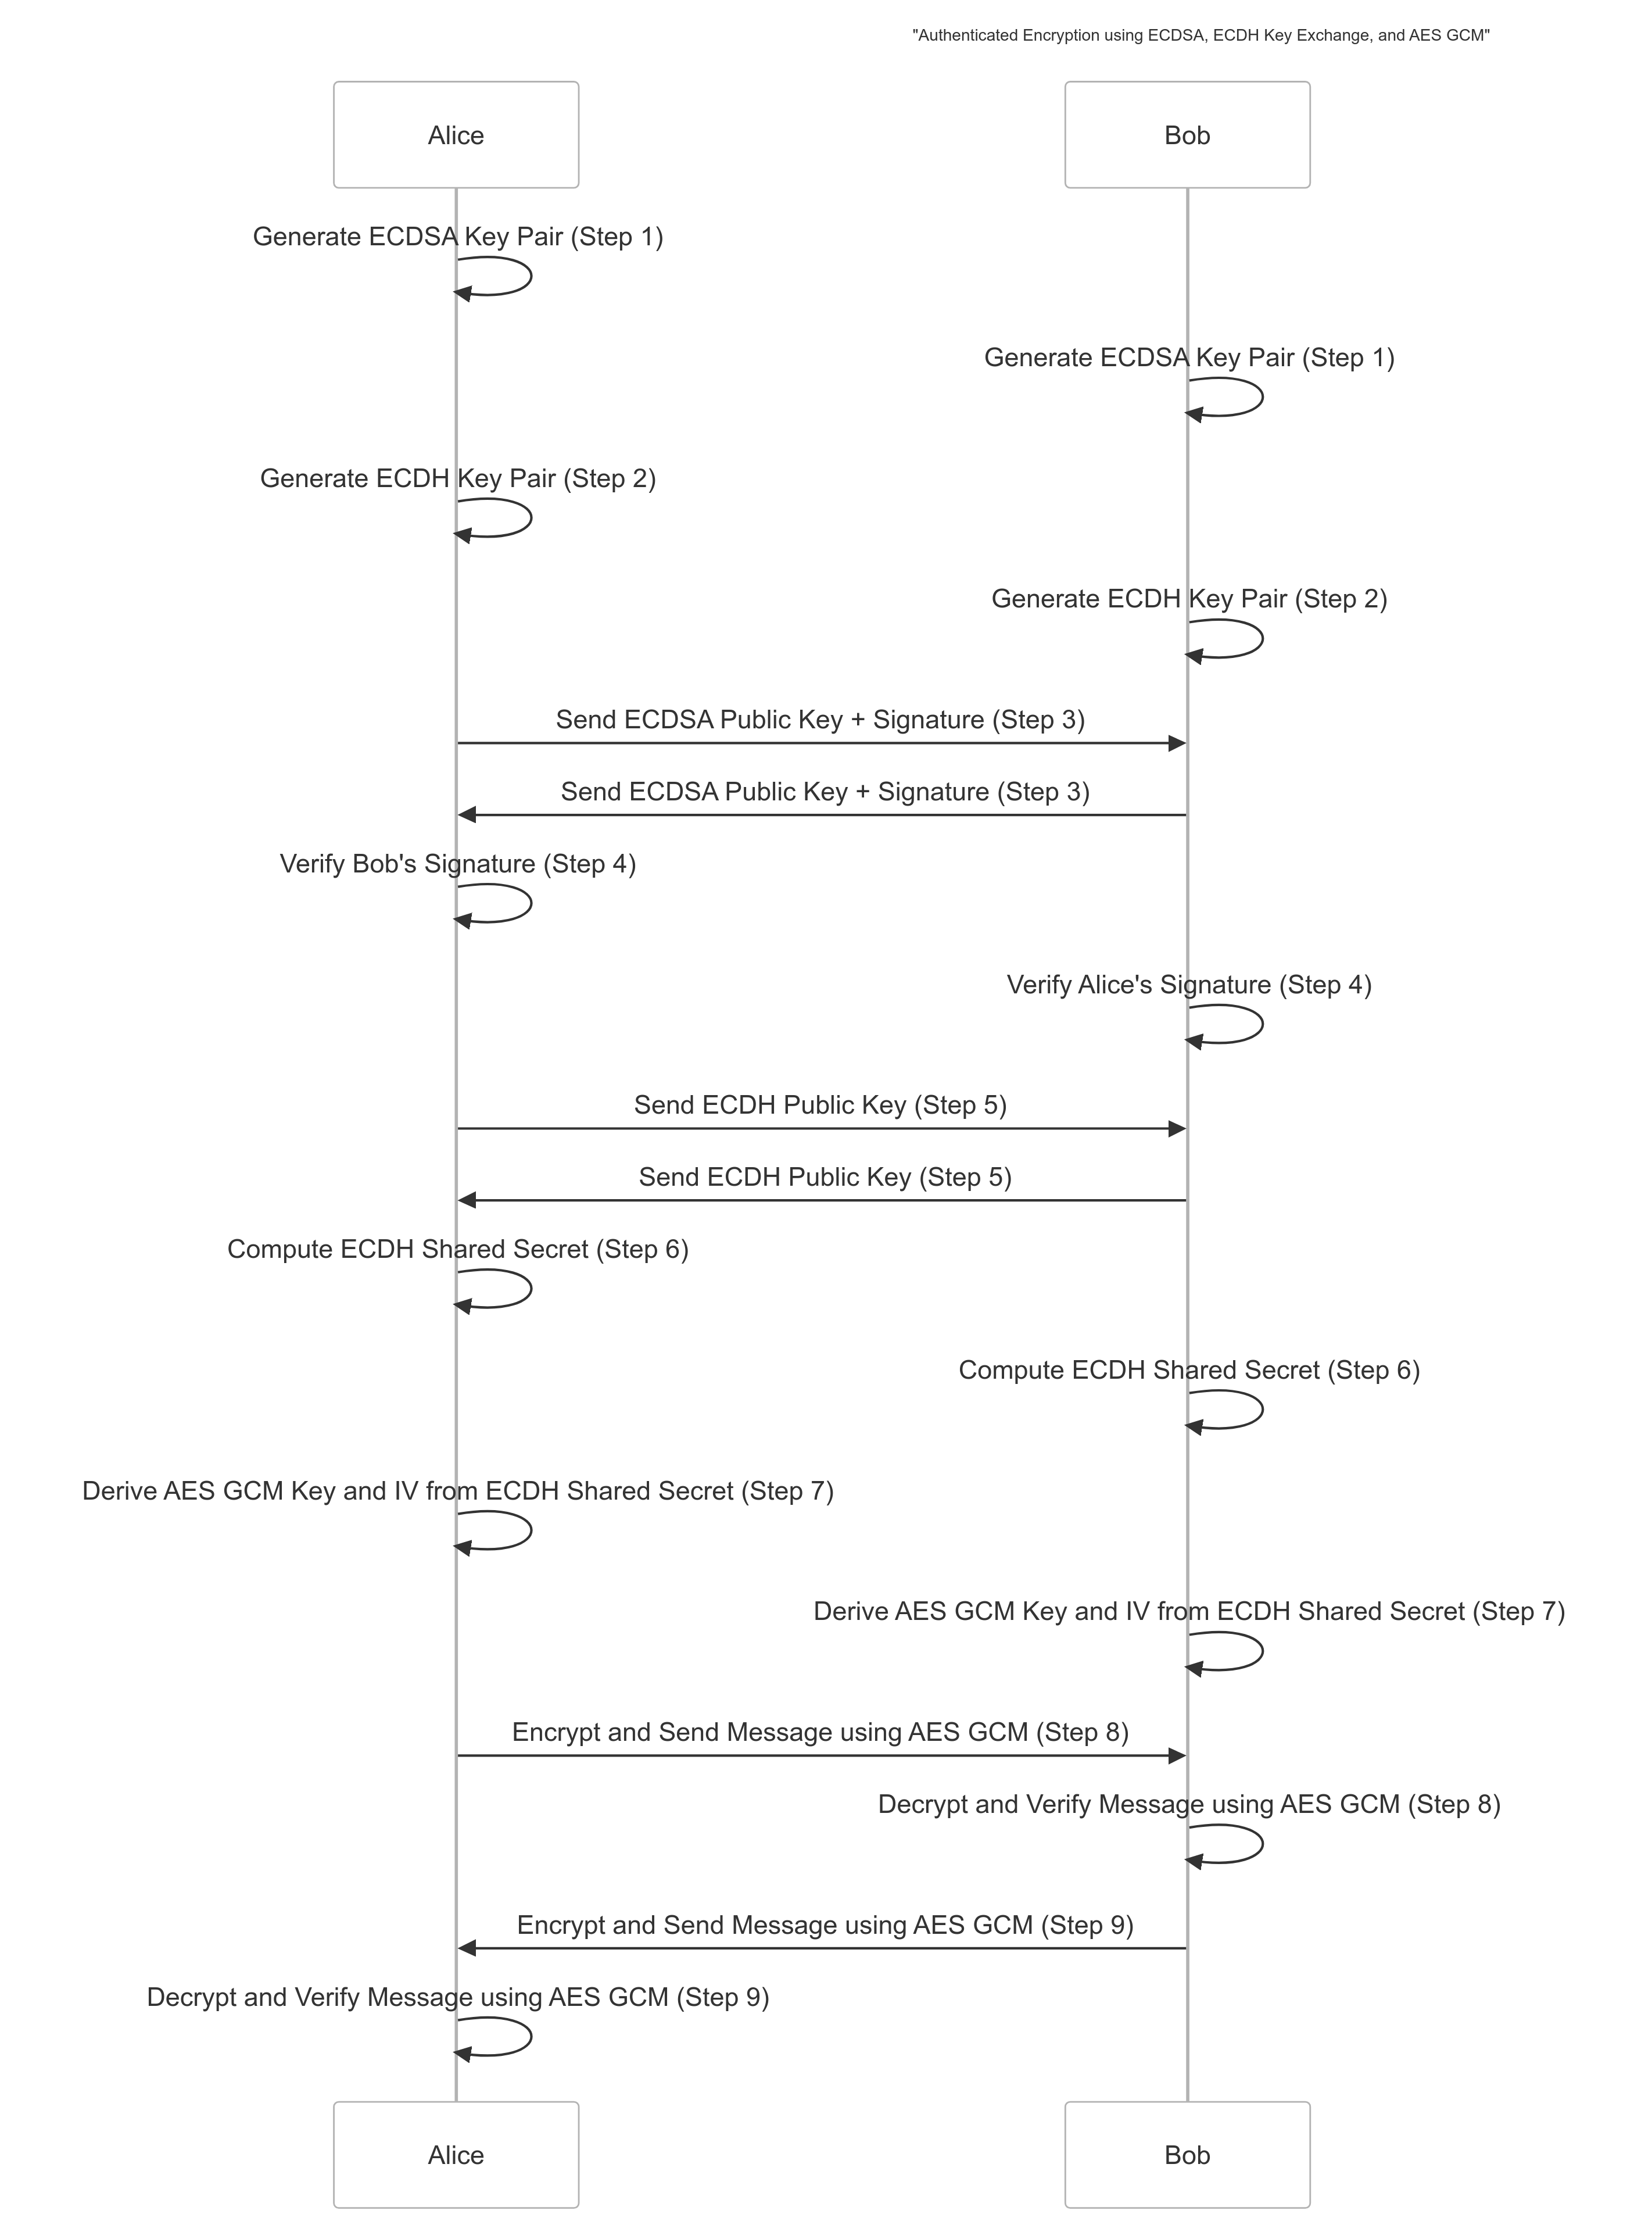
\includegraphics[width=17cm]{img/numbered auth enc.png}
  \caption{Sequence Diagram for "CryptoEngine" Demo }
  \label{fig:sequence_diagram}
\end{figure}

\hspace{1cm}The Sequence Diagram in Figure \ref{fig:sequence_diagram} illustrates the process of authenticated encryption using ECDSA for authentication, ECDH for key exchange, and AES GCM for encryption. The diagram shows the interactions between two participants, Alice and Bob, as they perform cryptographic operations to securely exchange messages.

\textit{Note : In our demo, the STM32XX and STM32U545 MCUs will play the roles of Alice and Bob respectively.}



This sequence diagram demonstrates a secure communication process where both participants authenticate each other using ECDSA, establish a shared secret using ECDH, and securely exchange messages using AES GCM. The use of these cryptographic techniques ensures the confidentiality, integrity, and authenticity of the exchanged messages.

\section{Demonstration Details and Explanation}
For confidentiality reasons we will only detail the "Bob" side of the demo, since it is using the STM32U545 MCU.

\subsection{ECDSA Key Pair Generation}
This is the first step of the demo. It involves setting up PKA peripheral to generate the public ECDSA key.
    \subsubsection{PKA Peripheral Initialization}
        To compute ECDSA public key we need to set the PKA mode to "ECC Fp scalar multiplication", then we need to input the cryptographic parameters in the correct addresses in PKA RAM.
    \subsubsection{ECC Scalar Multiplication }
        To input cryptographic parameters in PKA RAM, we need to refer to the STM32U5 reference manual \cite{U5_Refman} where we can find the specifications for using ECC Fp scalar multiplication.
        The details of this operation can be found in Figure \ref{fig:PKA ECC}.

         This figure details the address and size of every cryptography parameter involved in ECC multiplication, which we are using at this level to compute the ECDSA public key.
 Note that in our demonstration, since we are using a 256-bit curve, the size labeled as EOS (ECC Operand Size) is equal to 320 bits which are 256 bits of actual data and 64 bits of zeros which are necessary when inputting certain data to PKA RAM, as mentioned in the reference manual for U5 \cite{U5_Refman}.

\begin{figure}[H]
    \centering
    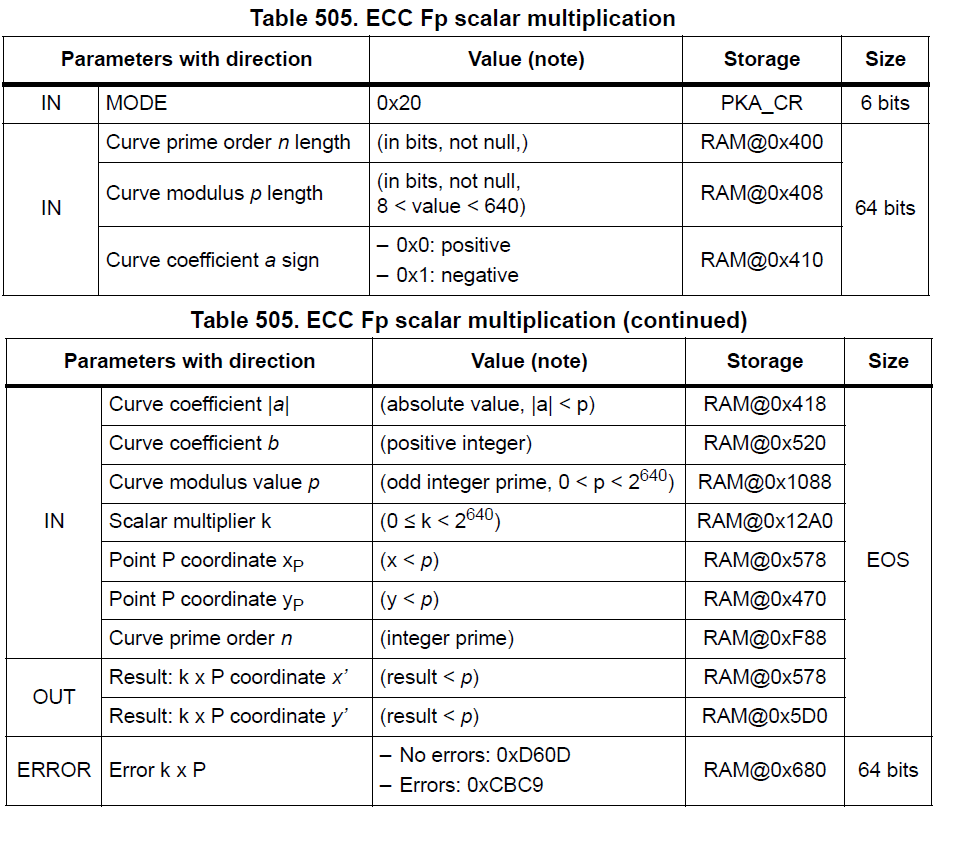
\includegraphics[width=15cm]{img/PKA ECC.png}
    \caption{PKA ECC Fp Scalar Multiplication}
    \label{fig:PKA ECC}
\end{figure}




 In our case the parameters that we need to use are provided by NIST \cite{Nist_curve} and are specified in the following table.

 
\begin{longtable}{|c|p{13cm}|}

\caption{NIST P-256 Curve Specifications} \\
\hline
\textbf{Name} & \textbf{Value} \\
\hline
\endfirsthead

\multicolumn{2}{c}%
{{\bfseries NIST P-256 Curve Specifications (continued)}} \\
\hline
\textbf{Name} & \textbf{Value} \\
\hline
\endhead

\hline \multicolumn{2}{|r|}{{Continued on next page}} \\ \hline
\endfoot

\hline \hline
\endlastfoot

Curve Modulus p & 0xffffffff00000001000000000000000000000000ffffffffffffffffffffffff \\
\hline
Curve Coefficient a & 0xffffffff00000001000000000000000000000000fffffffffffffffffffffffc \\
\hline
Curve Coefficient b & 0x5ac635d8aa3a93e7b3ebbd55769886bc651d06b0cc53b0f63bce3c3e27d2604b \\
\hline
Generator Point G & \begin{tabular}{@{}p{12cm}@{}} (0x6b17d1f2e12c4247f8bce6e563a440f277037d812deb33a0f4a13945d898c296, \\ 0x4fe342e2fe1a7f9b8ee7eb4a7c0f9e162bce33576b315ececbb6406837bf51f5) \end{tabular} \\
\hline
Curve prime order n & 0xffffffff00000000ffffffffffffffffbce6faada7179e84f3b9cac2fc632551 \\
\end{longtable}
\textit{Note : These same curve parameters will be reused for ECDSA signature generation and verification as well as ECDH key pair generation.
}

These curve specifications have to be put in their specific adresses in PKA RAM in order to set the stage for elliptic curve operations on the P-256 curve. 

Figure \ref{fig:curvo} demonstrates the code implementation of the curve parameters.


\begin{figure}[H]
    \centering
    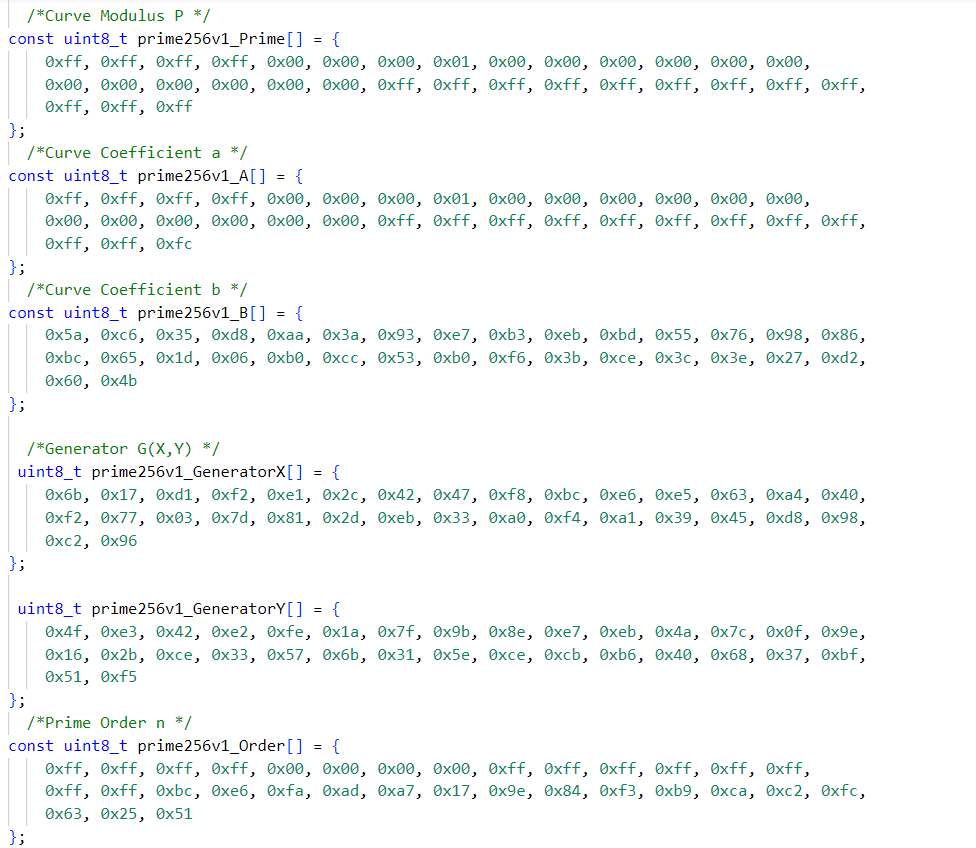
\includegraphics[width=19cm]{img/ecdsa curve params code.png}
    \caption{Code Implementation of NIST P-256 Parameters}
    \label{fig:curvo}
\end{figure}

We will use PKA structures provided by the Hardware Abstraction Layer (HAL) to configure our curve parameters, as illustrated in Figure \ref{fig:ecc struct}.
We have developed a function to fill in this structure's members with the NIST P-256 curve parameters as illustrated in Figure \ref{fig:pka_ecc_func}

\begin{figure}[H]
    \centering
    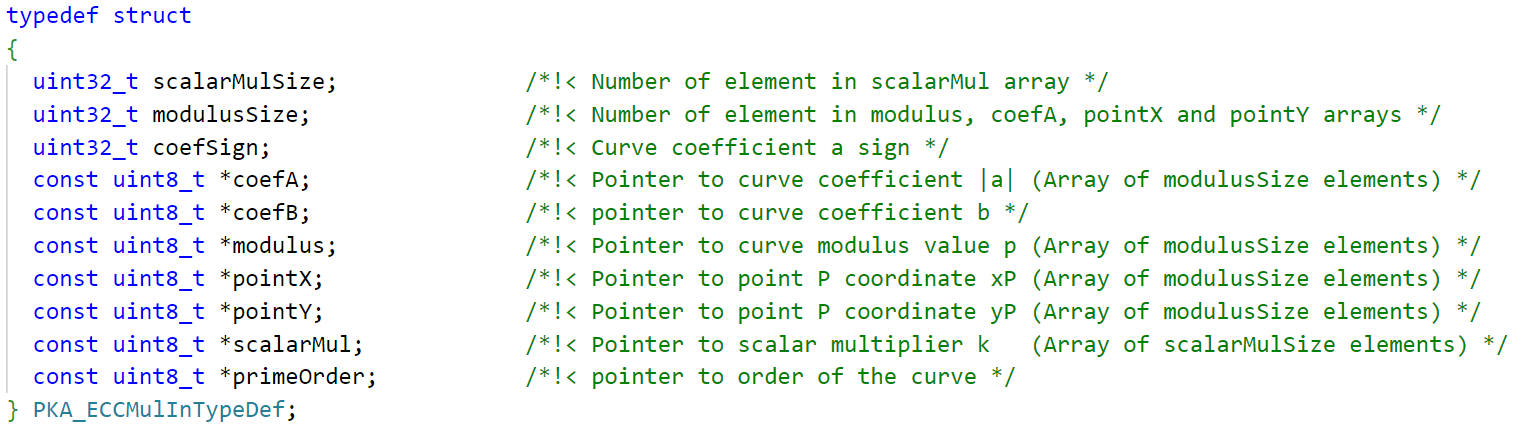
\includegraphics[width=18cm]{img/ecc struct.png}
    \caption{HAL PKA ECC Input Structure}
    \label{fig:ecc struct}
\end{figure}


\begin{figure}[H]
    \centering
    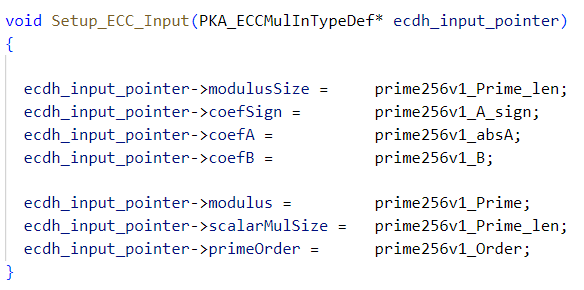
\includegraphics[width=15cm]{img/ecc func.png}
    \caption{PKA ECC Setup}
    \label{fig:pka_ecc_func}
\end{figure}

After setting up the elliptic curve parameters, we can generate the ECDSA public key using the ECDSA private key illustrated in Figure \ref{fig:ecdsa_priv_key}. Figure \ref{fig:pka_ecdsa_generate} shows the function used to generate the public key, and Figure \ref{fig:pka_pubkey_terminal1} shows the generated key, transmitted through USART to our terminal application. As previously mentioned in \ref{curve_param}, the ECDSA public key is a point on the elliptic curve which has a X and Y coordinate, each of them being 256 bits.

\begin{figure}[H]
    \centering
    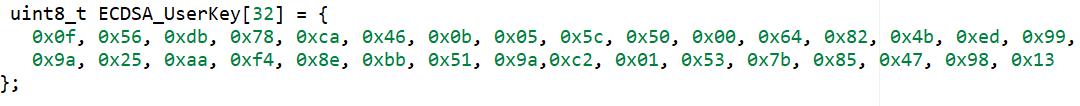
\includegraphics[width=18cm]{img/ecdsa priv key.png}
    \caption{ECDSA Private Key}
    \label{fig:ecdsa_priv_key}
\end{figure}


\begin{figure}[H]
    \centering
    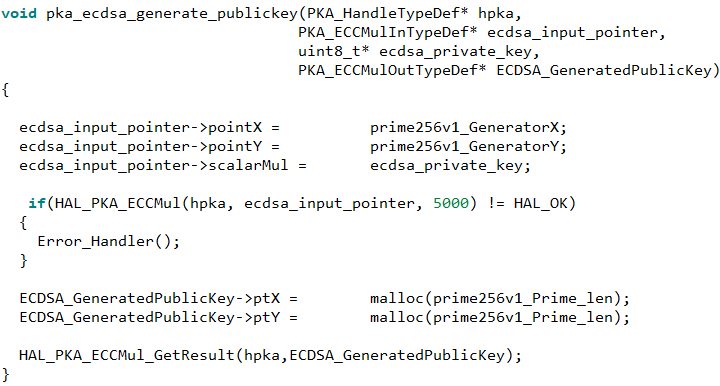
\includegraphics[width=16cm]{img/pka_generate_ecdsa.png}
    \caption{ECDSA Public Key Generation Function}
    \label{fig:pka_ecdsa_generate}
\end{figure}





\begin{figure}[H]
    \centering
    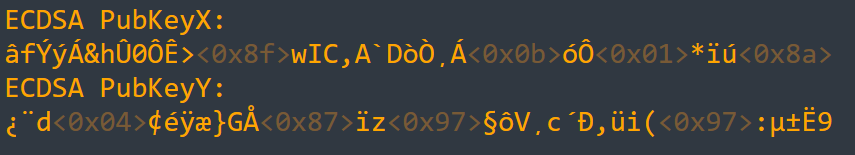
\includegraphics[width=15cm]{img/ecdsa pubkey.png}
    \caption{Generated ECDSA Public Key}
    \label{fig:pka_pubkey_terminal1}
\end{figure}

\subsection{ECDH Key Pair Generation}
This is the second step of the demo. Similarly to the previous step, we will use PKA to generate the ECDH public key.

    \subsubsection{ECC Scalar Multiplication}
    The key generation process using "ECC Fp scalar multiplication" is the same for ECDSA and ECDH, as described in Figure \ref{fig:PKA ECC}. We will use the same PKA structure as in ECDSA key generation as illustrated in Figure \ref{fig:ecc struct}.

    The ECDH private key illustrated in Figure \ref{fig:ecdh_priv} is used along with the function shown in Figure \ref{fig:ecc_generate} in order to generate the ECDH public key, which is shown in Figure \ref{fig:ecc_pub}.
    \begin{figure}[H]
    \centering
    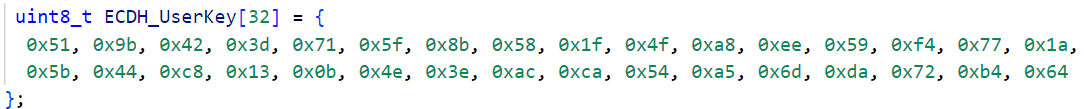
\includegraphics[width=15cm]{img/ecdh private}
    \caption{ECDH Private Key}
    \label{fig:ecdh_priv}
    \end{figure}

    \begin{figure}[H]
    \centering
    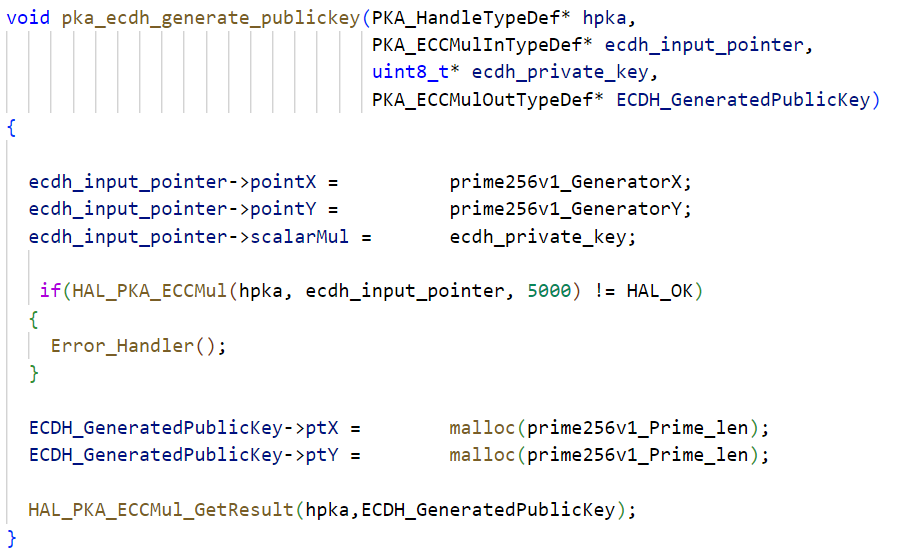
\includegraphics[width=13cm]{img/ecdh generate.png}
    \caption{ECDH Public Key Generation Function}
    \label{fig:ecc_generate}
    \end{figure}

    \begin{figure}[H]
    \centering
    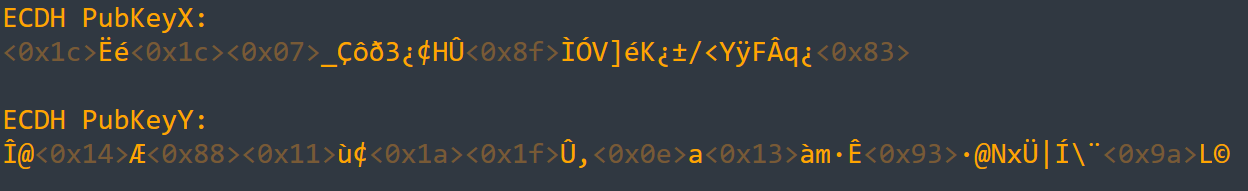
\includegraphics[width=13cm]{img/ecdh pub key.png}
    \caption{Generated ECDH Public Key }
    \label{fig:ecc_pub}
    \end{figure}

\subsection{ECDSA Signature Generation}    
%In order to ensure authenticity of the message exchange, we need to generate an ECDSA signature that will be sent along with the ECDSA public key to be used for signature verification.

To generate an ECDSA signature, we will use the PKA mode illustrated in Figure \ref{fig:ecdsa_sign_tab} \cite{U5_Refman}.
 \begin{figure}[H]
    \centering
    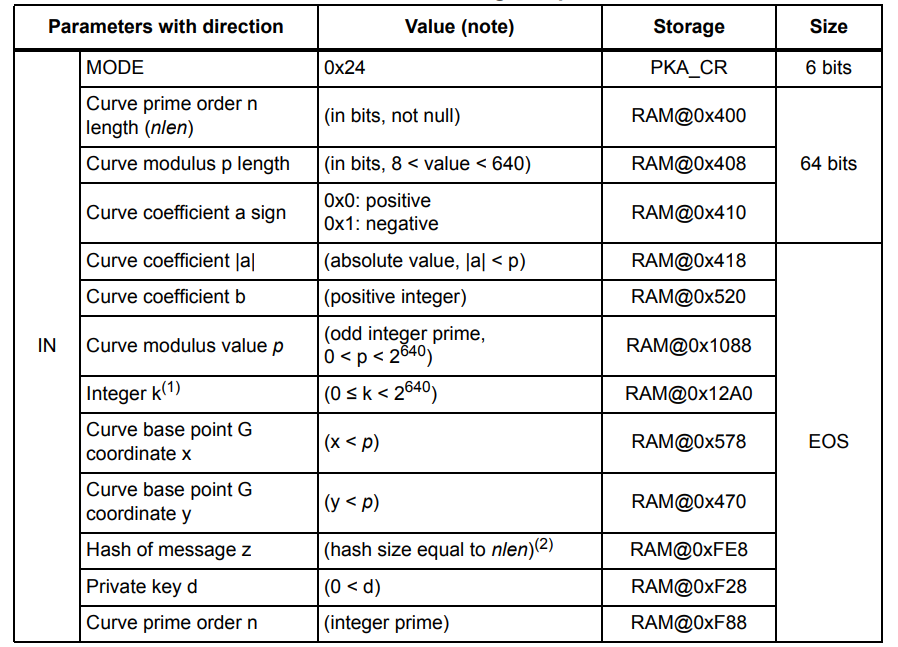
\includegraphics[width=14cm]{img/ecdsa sign2.png}
    \caption{ECDSA Sign Operation }
    \label{fig:ecdsa_sign_tab}
    \end{figure}

 We will use the PKA ECDSA signature structure provided by the HAL driver shown in Figure \ref{fig:ecdsa struct} along with the function shown in \ref{fig:ecdsa func} to input the signature parameters in PKA RAM.

\begin{figure}[H]
    \centering
    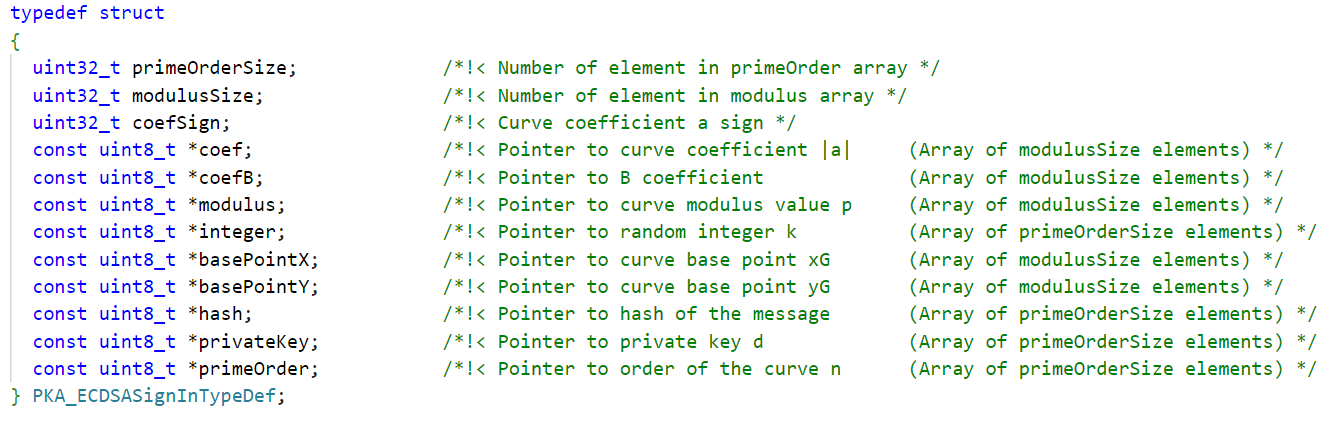
\includegraphics[width=17cm]{img/ecdsa struct.png}
    \caption{HAL PKA ECDSA Input Structure}
    \label{fig:ecdsa struct}
    \end{figure}

    \begin{figure}[H]
    \centering
    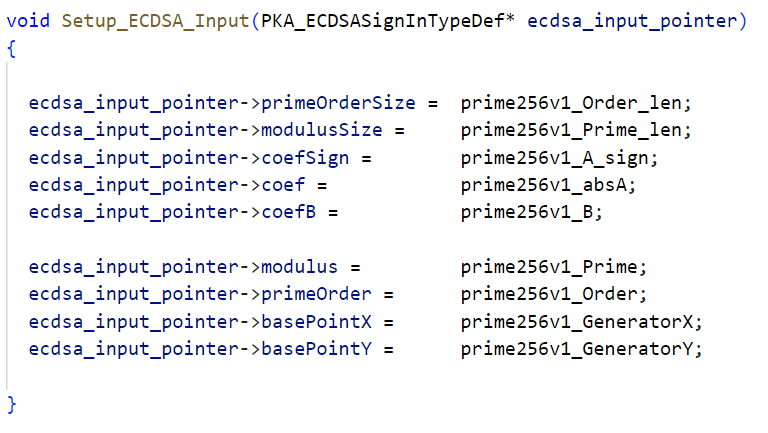
\includegraphics[width=17cm]{img/ecdsa_func.png}
    \caption{HAL PKA ECDSA Input Structure}
    \label{fig:ecdsa func}
    \end{figure}

    Compared to public key generation, generating the signature requires a new private parameter called "k" which is a 256-bit number only used once to generate the signature. The integer "k" used for this demo is shown in Figure \ref{fig:ecdsa_k}. The signature generation also uses a hash message, which in our demonstration is pre-shared between the two parties.
    \begin{figure}[H]
    \centering
    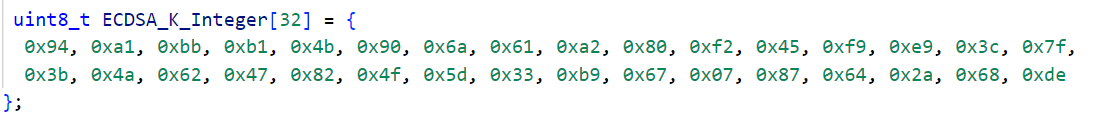
\includegraphics[width=17cm]{img/ecdsa k.png}
    \caption{ECDSA Integer "K"}
    \label{fig:ecdsa_k}
    \end{figure}
    After setting up the ECDSA HAL structure, we can launch the ECDSA signing operation using the function shown in Figure \ref{fig:ecdsa func2}.
    \begin{figure}[H]
    \centering
    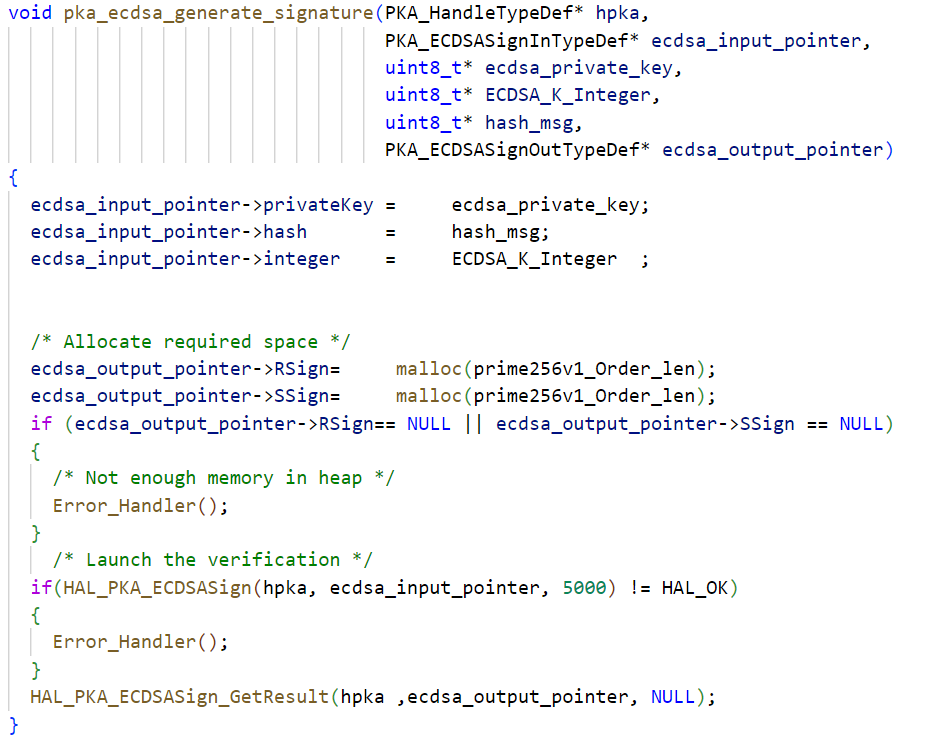
\includegraphics[width=17cm]{img/ecdsa func2.png}
    \caption{ECDSA Signing Function}
    \label{fig:ecdsa func2}
    \end{figure}

    The generated signature is composed of two parts "Signature R" and "Signature S", each being 256 bits long. Figure \ref{fig:ecdsa_rs} shows the output of the signing operation.
    
    \begin{figure}[H]
    \centering
    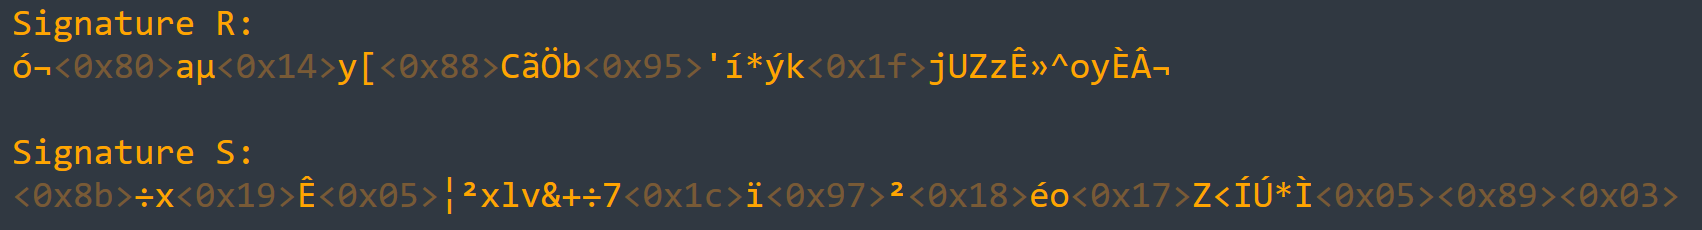
\includegraphics[width=17cm]{img/signature rs.png}
    \caption{Generated ECDSA Signature}
    \label{fig:ecdsa_rs}
    \end{figure}

    \subsection{ECDSA Public Key and Signature Exchange}
    After having generated the ECDSA public keys and signatures, the two MCUs exchange these parameters using USART. Exchanging these parameters is crucial for the following step, which is signature verification, to ensure the authenticity of the communication.
    
    Figure \ref{fig:received sign} shows the ECDSA public key and signature received by "Bob" which were generated by "Alice". 
    \begin{figure}[H]
    \centering
    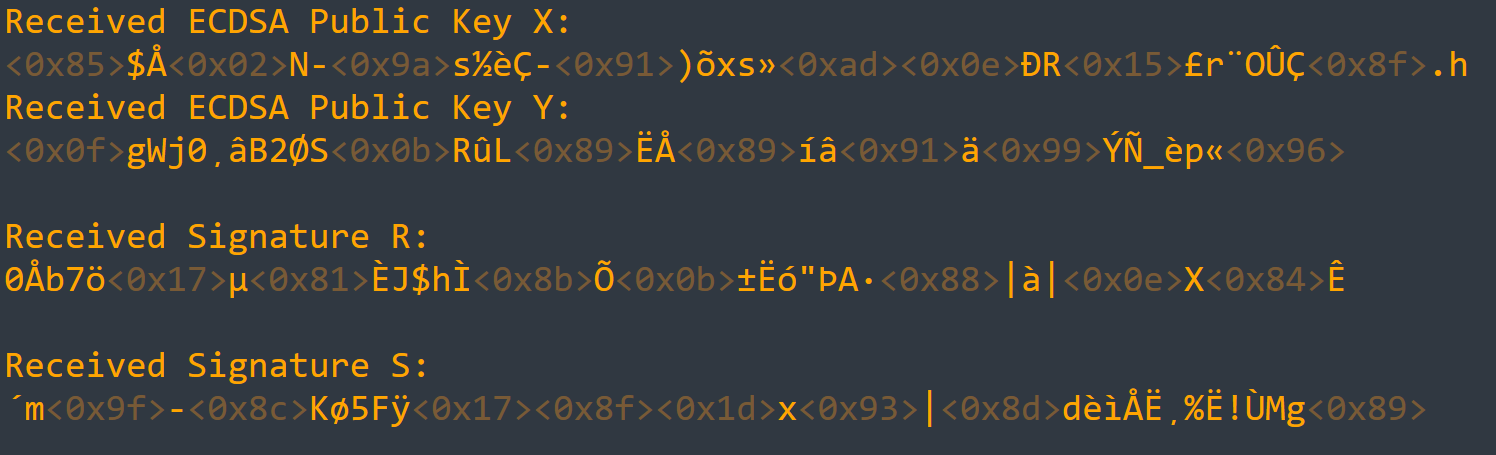
\includegraphics[width=16cm]{img/received sigpub.png}
    \caption{Received ECDSA Signature}
    \label{fig:received sign}
    \end{figure}

    \subsection{ECDSA Signature Verification}
    In this step, each device verifies the ECDSA signature sent by the other party using the PKA mode "ECDSA Verification" shown in Figure \ref{fig:ecdsa verif} \cite{U5_Refman}.
    A lot of the same curve parameters are the same as ECDSA signature generation , with the addition of the received public key and signature parameters.
    \begin{figure}[H]
    \centering
    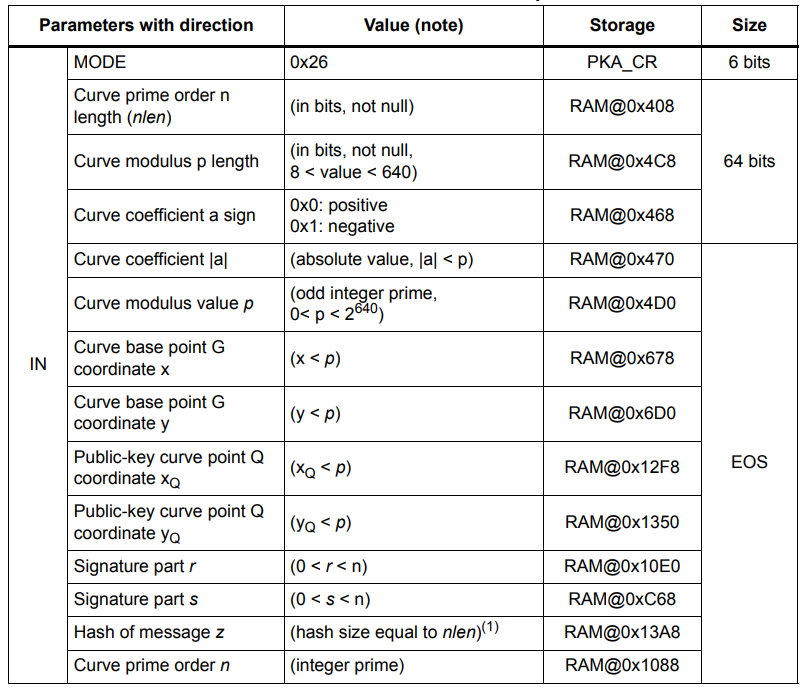
\includegraphics[width=16cm]{img/ecdsa verify.png}
    \caption{PKA "ECDSA Verification" Mode}
    \label{fig:ecdsa verif}
    \end{figure}

    Figure \ref{fig:ecdsa verif func} shows the code implementation of the ECDSA signature verification process.
    \begin{figure}[H]
    \centering
    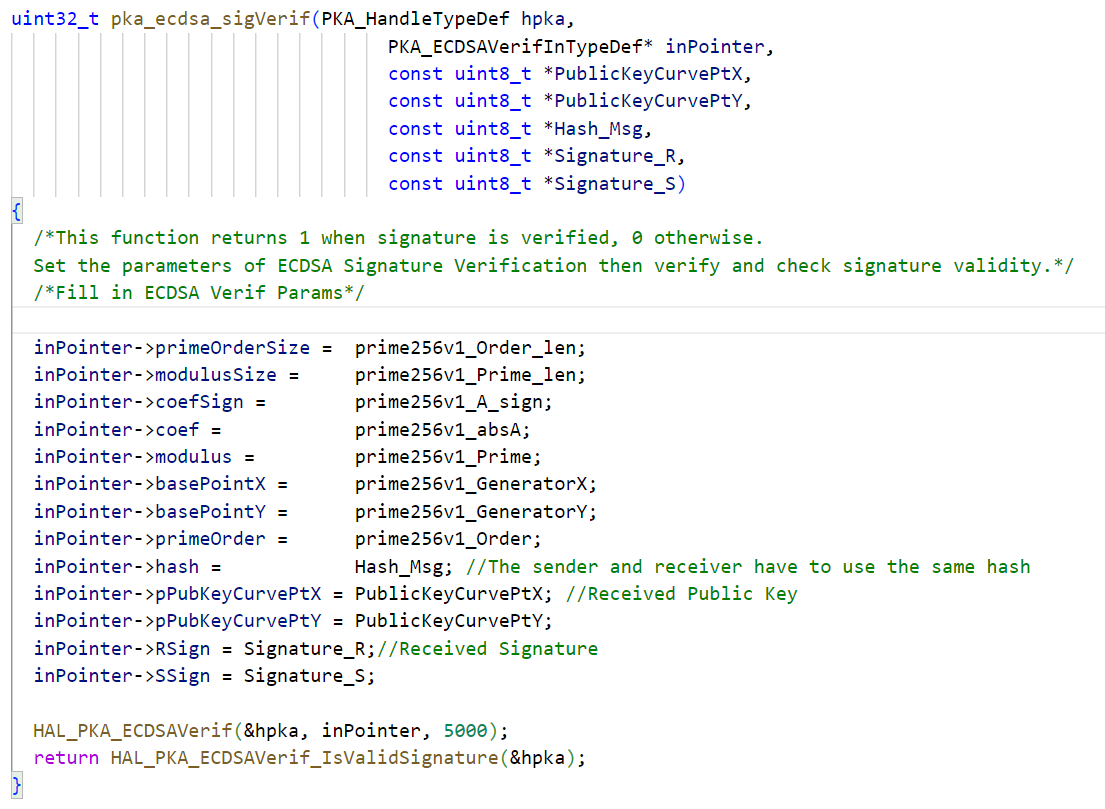
\includegraphics[width=18cm]{img/ecdsa verif func.png}
    \caption{ECDSA Verification Function }
    \label{fig:ecdsa verif func}
    \end{figure}
    
   There are two outcomes to signature verification. Figure \ref{fig:verif out} shows the output of a successful signature verification process, which allows to go on to establish ECDH key exchange, while Figure \ref{fig:ecdsa verif fail} shows the output of a failed signature verification which abruptly ends the communication. 
   
   \begin{figure}[H]
    \centering
    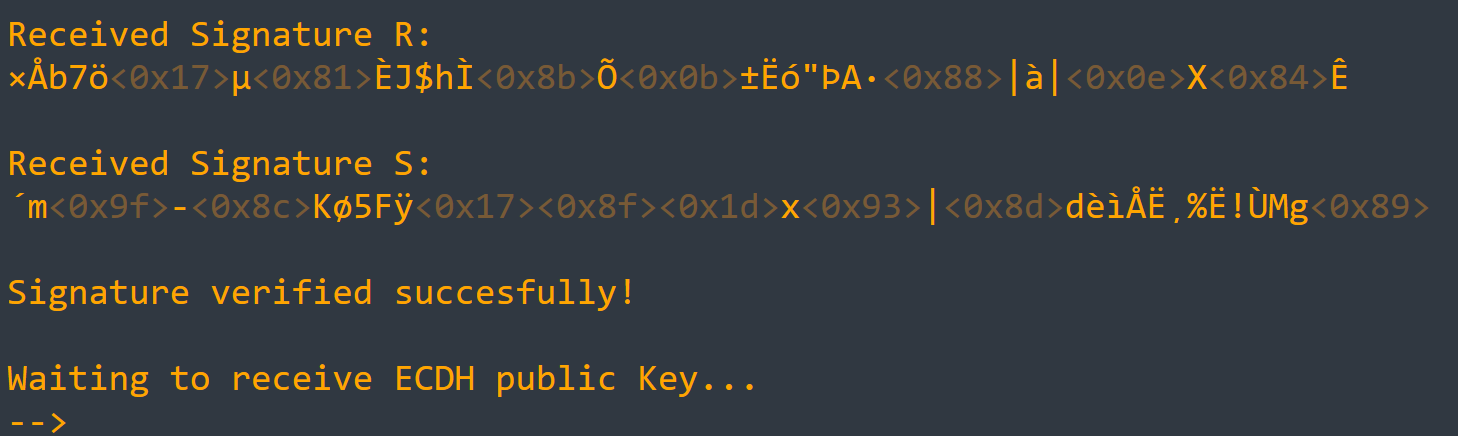
\includegraphics[width=18cm]{img/verif out.png}
    \caption{Successful ECDSA Signature Verification}
    \label{fig:verif out}
    \end{figure}
    
    \begin{figure}[H]
    \centering
    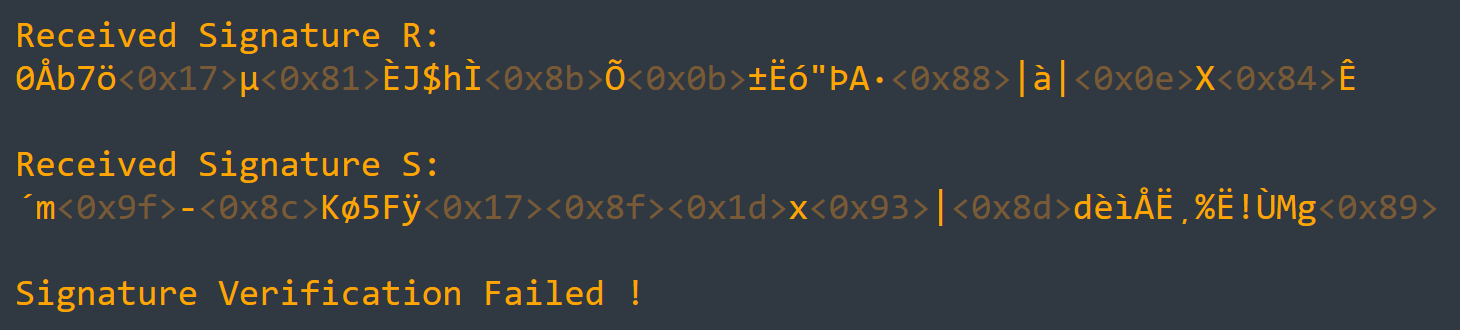
\includegraphics[width=18cm]{img/verif fail.png}
    \caption{Failed ECDSA Signature Verification}
    \label{fig:ecdsa verif fail}
    \end{figure}

    \subsection{ECDH Public Key Exchange}
    Now that the two parties have verified each other's signature, we can proceed knowing that authenticity has been assured. The next step is to establish a shared secret which will serve as a basis for establishing a symmetric encryption key. For that, the two devices must exchange the ECDH public keys generated at the start of the demo via USART. Figure \ref{fig:ecdh_pub} shows the terminal output of the ECDH public key reception process.
    
    \begin{figure}[H]
    \centering
    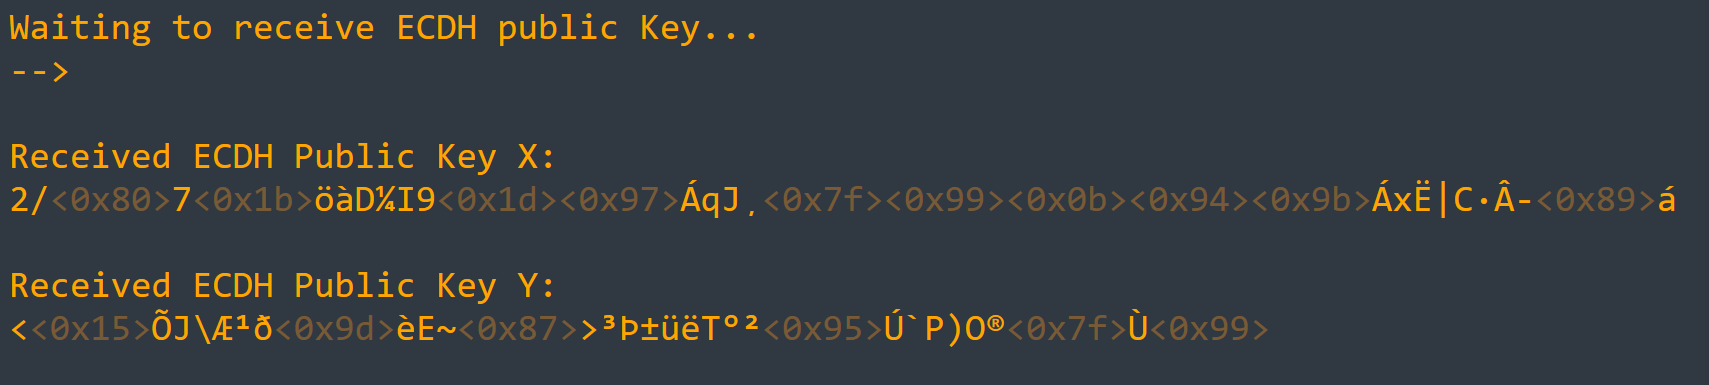
\includegraphics[width=17cm]{img/received ecdh pub.png}
    \caption{Received ECDH Public Key}
    \label{fig:ecdh_pub}
    \end{figure}
    
    \subsection{ECDH Shared Secret Generation}
    Having exchanged the ECDH public keys, each device will independently calculate the ECDH shared secret which will be a point on the elliptic curve. This point is obtained through multiplying the device's own ECDH private key with the received ECDH public key. Naturally, both devices should obtain the same common 512-bit shared secret.

    Shared secret generation is done through ECC scalar multiplication, meaning we will use the PKA mode "ECC Fp scalar multiplication" which has been detailed in Figure \ref{fig:PKA ECC} \cite{U5_Refman}.

    Figure \ref{fig:shared sec} illustrates the code implementation of ECDH shared secret generation, and Figure \ref{fig:shared sec out} shows the output result of this operation.
    \begin{figure}[H]
    \centering
    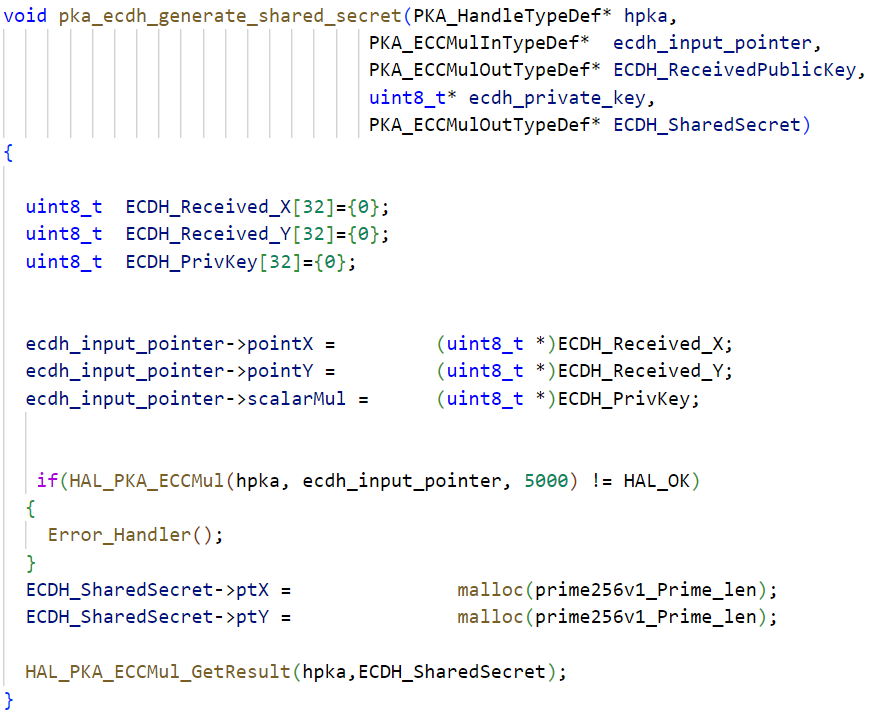
\includegraphics[width=17cm]{img/shared sec.png}
    \caption{ECDH Shared Secret Generation Function}
    \label{fig:shared sec}
    \end{figure}

    
    \begin{figure}[H]
    \centering
    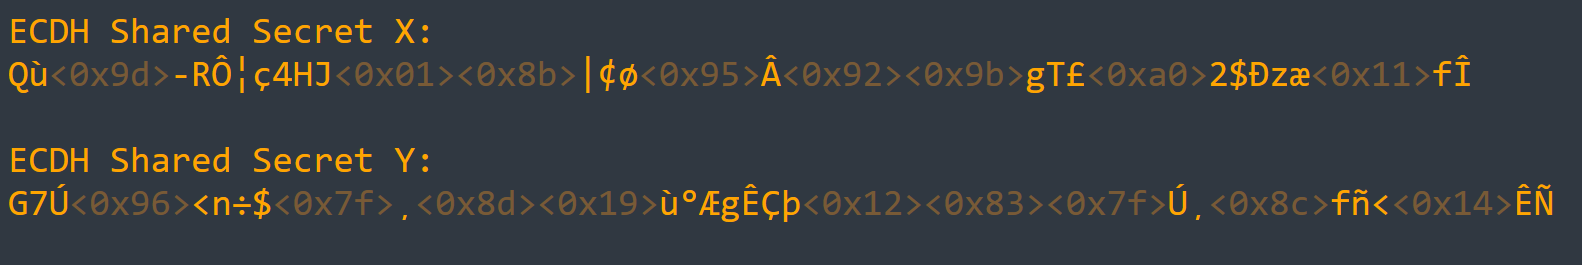
\includegraphics[width=17cm]{img/shared sec out.png}
        \caption{ECDH Shared Secret}
    \label{fig:shared sec out}
    \end{figure}
    \subsection{AES GCM Key and IV Derivation}
    Having established the shared secret, we will now derive from it the symmetric encryption key as well as the initialization vector which are needed for AES GCM .
    Usually, this process would involve a key derivation function and the use of complicated algorithms, but for the purposes of the simplicity of the demo  we opted to take the X coordinate of the ECDH shared secret as the 256-bit AES Key and the first 96 bits of the Y coordinate as the initialization vector.
    \subsection{AES GCM Symmetric Encryption}
    For this step, we will use the AES peripheral structure provided by the HAL driver provided in Figure \ref{fig:aes struct}. We will initialize the peripheral's structure as shown in Figure \ref{fig:aes init}, where we select a 256-bit key size and AES GCM mode.
    \begin{figure}[H]
    \centering
    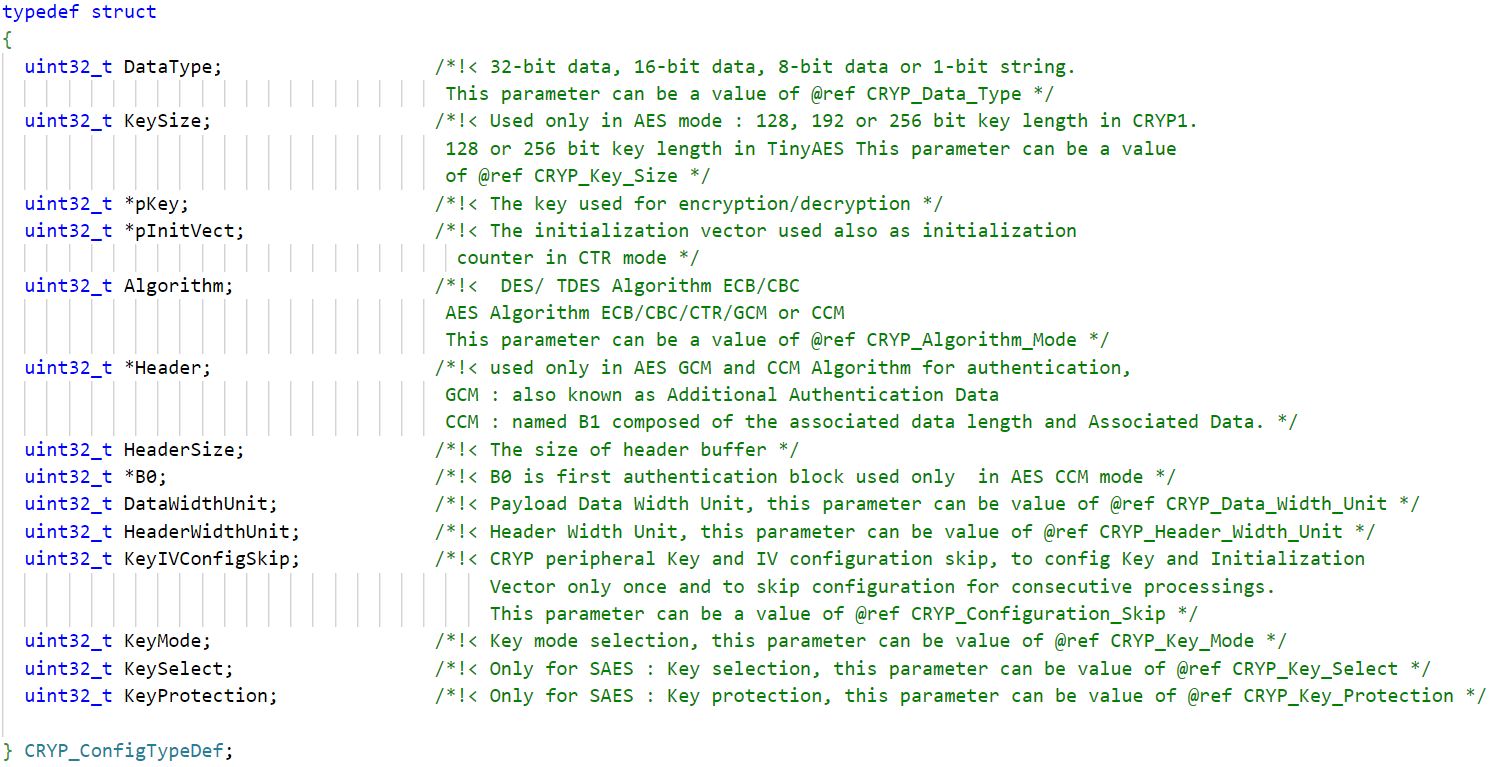
\includegraphics[width=18cm]{img/aes struct.png}
        \caption{AES HAL Structure}
    \label{fig:aes struct}
    \end{figure}

    \begin{figure}[H]
    \centering
    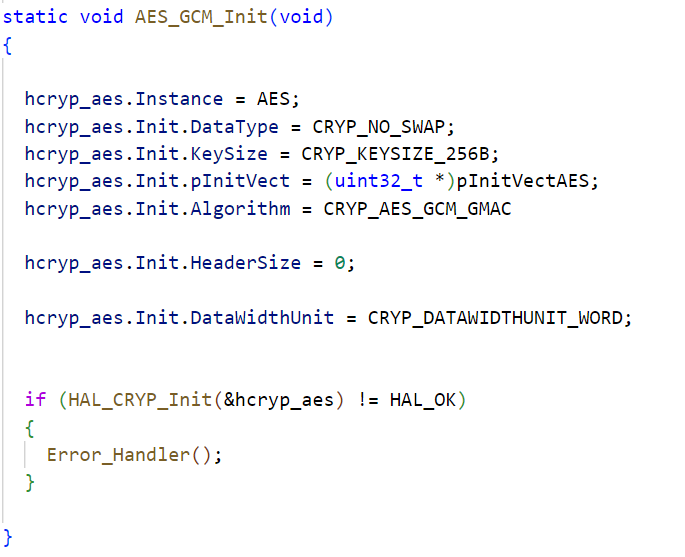
\includegraphics[width=10cm]{img/aes init.png}
        \caption{AES Structure Initialization}
    \label{fig:aes init}
    \end{figure}

    All that is left is to derive the AES key and initialization vector from the ECDH shared secret as shown in Figure \ref{fig:deriv}.
    
    \begin{figure}[H]
    \centering
    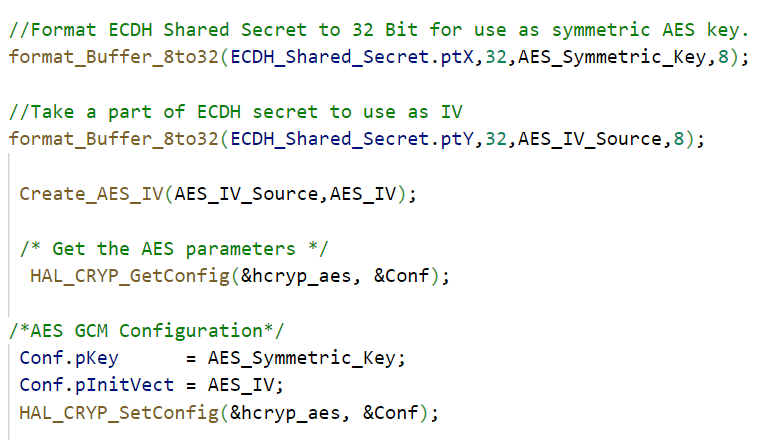
\includegraphics[width=12cm]{img/deriv.png}
        \caption{AES GCM Key and Initialization Vector Derivation}
    \label{fig:deriv}
    \end{figure}

    On the "Bob" side, we will encrypt and send the message "This is Bob" along with the tag that will help in verifying the integrity of the message. Figure \ref{fig:bob hello} demonstrates the plaintext, ciphertext and tag generated by the encryption process. Note that the "\%" symbol was added for extra padding since the AES peripheral expects a 128-bit input.

    \begin{figure}[H]
    \centering
    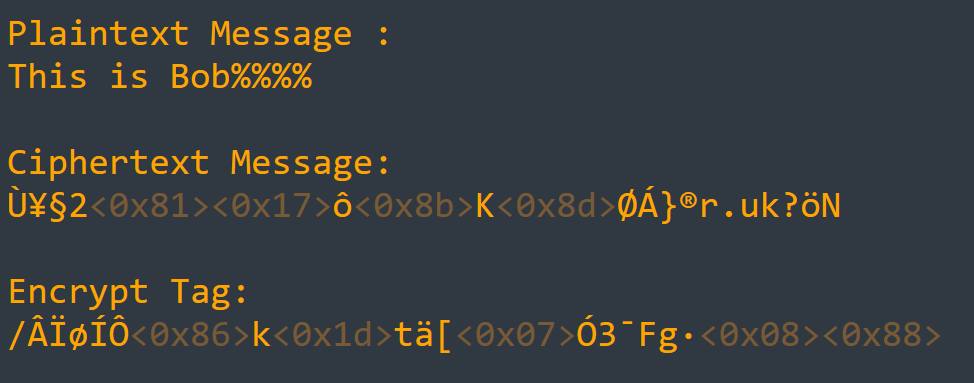
\includegraphics[width=12cm]{img/bob hello.png}
        \caption{AES GCM Key and Initialization Vector Derivation}
    \label{fig:bob hello}
    \end{figure}

    \subsection{Message Decryption and Tag Verification}
    The two devices exchange the encrypted messages and the generated tags. They must now decrypt the message while regenrating a tag. If the received tag is the same as the generated decryption tag, that means the message has been decrypted succesfully. Figure \ref{fig:tag} shows the decryption process on the "Bob" side which shows the correct decryption of the "Alice" message ("This is Alice").
    
    \begin{figure}[H]
    \centering
    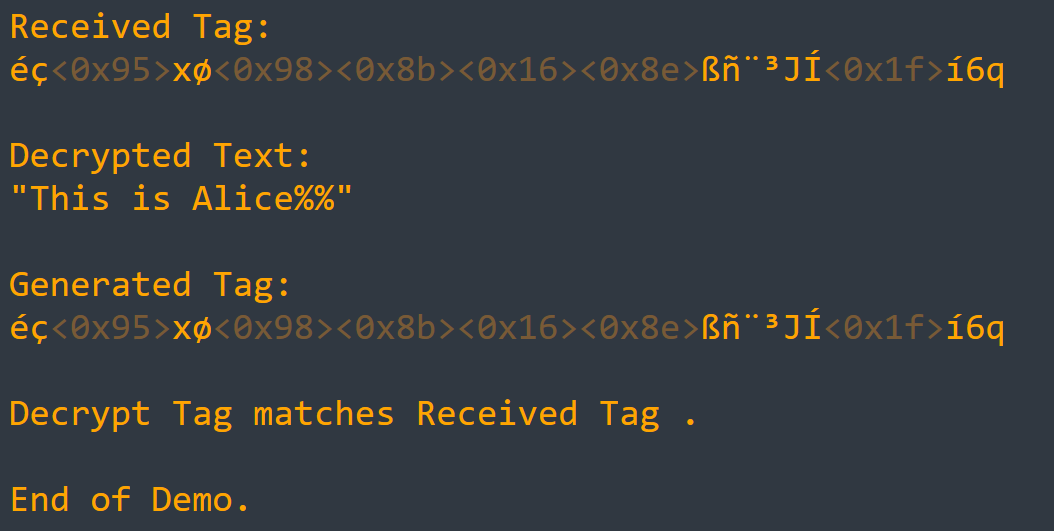
\includegraphics[width=14cm]{img/end of demo.png}
        \caption{Message Decryption Output}
    \label{fig:tag}
    \end{figure}
The matching of the tags proves that the message was transmitted correctly and without any manipulation. It also ensures that the two sides have managed to derive the exact same symmetric key from the shared secret generation process, meaning that a secure line of communication has been succesfully established between the two devices.
\section*{Conclusion}
This chapter provided a comprehensive review of the implementation steps for the "CryptoEngine" demo, which demonstrates secure communication between two microcontrollers using cryptographic techniques. We explored the generation and exchange of cryptographic keys, including ECDSA and ECDH keys, and the processes of signature generation, verification, and secure message exchange using AES GCM. We also included relevant code snippets and expected outputs for each step of the demonstration to provide a complete overview.